\section{Date: 2026-11-27}
\noindent \textbf{Series ID: EALOXSSNQ} 

\noindent This series is titled Average Loan Size for More than 365 Days, Other Risk (Acceptable), Small Domestic Banks (DISCONTINUED) and has a frequency of Quarterly, 2nd Month's 1st Full Week. The units are Thousands of Dollars and the seasonal adjustment is Not Seasonally Adjusted.The observation start date is 1997-04-01 and the observation end date is 2017-04-01.The popularity of this series is 1. \\ 

\noindent \textbf{Series ID: M1NTOTL1EQ000} 

\noindent This series is titled Current-Cost Depreciation of Fixed Assets: Private: Nonresidential: Equipment and has a frequency of Annual. The units are Millions of Dollars and the seasonal adjustment is Not Seasonally Adjusted.The observation start date is 1925-01-01 and the observation end date is 2024-01-01.The popularity of this series is 2. \\ 

\subsection{Raw Regression}
\noindent Regresses the two series against each other directly. A significant result here can come just as easily from both series sharing a long-run trend as from any real relationship.

\begin{center}
\begin{tabular}{lclc}
\toprule
\textbf{Dep. Variable:}         & value\_fred\_M1NTOTL1EQ000 & \textbf{  R-squared:         } &     0.006   \\
\textbf{Model:}                 &            OLS             & \textbf{  Adj. R-squared:    } &    -0.050   \\
\textbf{Method:}                &       Least Squares        & \textbf{  F-statistic:       } &    0.1028   \\
\textbf{Date:}                  &      Fri, 27 Nov 2026      & \textbf{  Prob (F-statistic):} &    0.752    \\
\textbf{Time:}                  &          20:24:12          & \textbf{  Log-Likelihood:    } &   -264.76   \\
\textbf{No. Observations:}      &               20           & \textbf{  AIC:               } &     533.5   \\
\textbf{Df Residuals:}          &               18           & \textbf{  BIC:               } &     535.5   \\
\textbf{Df Model:}              &                1           & \textbf{                     } &             \\
\textbf{Covariance Type:}       &         nonrobust          & \textbf{                     } &             \\
\bottomrule
\end{tabular}
\begin{tabular}{lcccccc}
                                & \textbf{coef} & \textbf{std err} & \textbf{t} & \textbf{P$> |$t$|$} & \textbf{[0.025} & \textbf{0.975]}  \\
\midrule
\textbf{const}                  &    6.933e+05  &      7.2e+04     &     9.623  &         0.000        &     5.42e+05    &     8.45e+05     \\
\textbf{value\_fred\_EALOXSSNQ} &    -142.6743  &      444.937     &    -0.321  &         0.752        &    -1077.451    &      792.103     \\
\bottomrule
\end{tabular}
\begin{tabular}{lclc}
\textbf{Omnibus:}       &  1.835 & \textbf{  Durbin-Watson:     } &    0.053  \\
\textbf{Prob(Omnibus):} &  0.399 & \textbf{  Jarque-Bera (JB):  } &    1.042  \\
\textbf{Skew:}          &  0.161 & \textbf{  Prob(JB):          } &    0.594  \\
\textbf{Kurtosis:}      &  1.930 & \textbf{  Cond. No.          } &     364.  \\
\bottomrule
\end{tabular}
%\caption{OLS Regression Results}
\end{center}

Notes: \newline
 [1] Standard Errors assume that the covariance matrix of the errors is correctly specified.

\begin{figure}
\centering
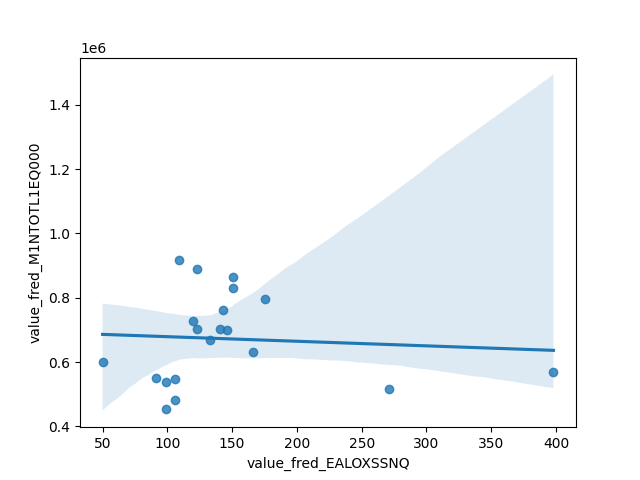
\includegraphics[scale = 0.9]{plots/plot_2026-11-27.png}
\caption{Raw Regression Plot for 2026-11-27}
\end{figure}
\newpage
\subsection{Detrended Regression}
\noindent Regresses the residuals of each series after removing its own linear time trend, so a shared trend can no longer drive the result on its own. A relationship that stays significant here is better evidence of a genuine link between the two series.

\begin{center}
\begin{tabular}{lclc}
\toprule
\textbf{Dep. Variable:}                    & value\_fred\_M1NTOTL1EQ000\_detrended & \textbf{  R-squared:         } &     0.014   \\
\textbf{Model:}                            &                  OLS                  & \textbf{  Adj. R-squared:    } &    -0.041   \\
\textbf{Method:}                           &             Least Squares             & \textbf{  F-statistic:       } &    0.2602   \\
\textbf{Date:}                             &            Fri, 27 Nov 2026           & \textbf{  Prob (F-statistic):} &    0.616    \\
\textbf{Time:}                             &                20:24:12               & \textbf{  Log-Likelihood:    } &   -221.82   \\
\textbf{No. Observations:}                 &                     20                & \textbf{  AIC:               } &     447.6   \\
\textbf{Df Residuals:}                     &                     18                & \textbf{  BIC:               } &     449.6   \\
\textbf{Df Model:}                         &                      1                & \textbf{                     } &             \\
\textbf{Covariance Type:}                  &               nonrobust               & \textbf{                     } &             \\
\bottomrule
\end{tabular}
\begin{tabular}{lcccccc}
                                           & \textbf{coef} & \textbf{std err} & \textbf{t} & \textbf{P$> |$t$|$} & \textbf{[0.025} & \textbf{0.975]}  \\
\midrule
\textbf{const}                             &   -2.266e-09  &     3739.682     & -6.06e-13  &         1.000        &    -7856.781    &     7856.781     \\
\textbf{value\_fred\_EALOXSSNQ\_detrended} &     -26.5584  &       52.068     &    -0.510  &         0.616        &     -135.949    &       82.832     \\
\bottomrule
\end{tabular}
\begin{tabular}{lclc}
\textbf{Omnibus:}       &  2.255 & \textbf{  Durbin-Watson:     } &    0.552  \\
\textbf{Prob(Omnibus):} &  0.324 & \textbf{  Jarque-Bera (JB):  } &    1.251  \\
\textbf{Skew:}          & -0.276 & \textbf{  Prob(JB):          } &    0.535  \\
\textbf{Kurtosis:}      &  1.906 & \textbf{  Cond. No.          } &     71.8  \\
\bottomrule
\end{tabular}
%\caption{OLS Regression Results}
\end{center}

Notes: \newline
 [1] Standard Errors assume that the covariance matrix of the errors is correctly specified.

\begin{figure}
\centering
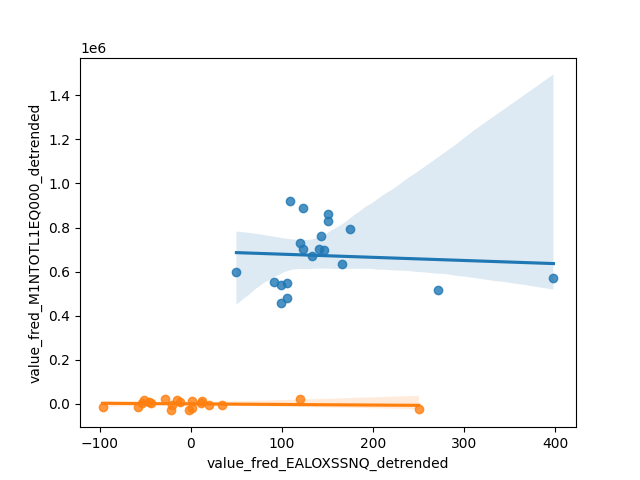
\includegraphics[scale = 0.9]{plots/plot_2026-11-27_detrended.png}
\caption{Detrended Regression Plot for 2026-11-27}
\end{figure}
\newpage
